% !TeX encoding=utf8
% !TeX spellcheck = de-DE

%%%%%%%%%%%%%%%%%%%%%%%%%%%%%%%%%% PACKAGES %%%%%%%%%%%%%%%%%%%%%%%%%%%%%%%%%%
\documentclass[
	pdftex,%              PDFTex verwenden
	a4paper,%             A4 Papier
	oneside,%             Einseitig
	bibtotoc,%    			Literaturverzeichnis einf�gen bibtotocnumbered: nummeriert
	liststotoc,%			Verzeichnisse einbinden in toc
	halfparskip,%        Europ�ischer Satz mit abstand zwischen Abs�tzen
	chapterprefix,%       Kapitel anschreiben als Kapitel
	headsepline,%         Linie nach Kopfzeile
	12pt%                 Gr�ssere Schrift, besser lesbar am bildschrim
]{scrartcl}


\usepackage[ngerman]{babel}
\usepackage[utf8x]{inputenc}
\usepackage[babel,french=guillemets,german=swiss]{csquotes} % Quotes
% Better Tables
\usepackage{array} 
\usepackage{tabularx}
\usepackage{booktabs}
\usepackage{graphicx} % Pictures
\usepackage{wrapfig}   
\usepackage[
	dvipsnames, % Load a set of predefined colors 
	table,      % Load the colortbl package
	hyperref,   % Support  the  hyperref  package
	fixinclude, % Prevent dvips color reset before .eps file inclusion
]{xcolor} % Colors in PDF

\usepackage[%
	automark,
	komastyle,
	nouppercase,
]{scrpage2}


\usepackage[savemem]{listings} % Listings (Code snippets)

\usepackage{amsmath}

\usepackage{vmargin}

\usepackage[%
	tocindentauto,     % all widths at the TOCs are calculated by tocindentauto
	tocgraduated,      % standard
	tocbreaksstrict,   % sets a lot of penalties before and after TOC entries 
	toctextentriesleft,   % indented as if they have an empty number.
]{tocstyle}

\usepackage[
	,backref=page       % Adds backlink text to the end of each item in the
	,pagebackref=false  % Adds backlink text to the end of each item in the
	,hyperindex=true    % Makes the page numbers of index entries into
hyperlinks.
	,hyperfootnotes=false % Makes the footnote marks into hyperlinks to the
	,bookmarks=true 
	,pdfpagelabels=true % set PDF page labels
]{hyperref}


\graphicspath{{images/}}



% ~~~~~~~~~~~~~~~~~~~~~~~~~~~~~~~~~~~~~~~~~~~~~~~~~~~~~~~~~~~~~~~~~~~~~~~~
% Configurations
% ~~~~~~~~~~~~~~~~~~~~~~~~~~~~~~~~~~~~~~~~~~~~~~~~~~~~~~~~~~~~~~~~~~~~~~~~
\setmarginsrb{2.6 cm}{1 cm}{2.6 cm}{2.5 cm}{1 cm}{1.5 cm}{1 cm}{1.5 cm}

%%% set layout of PDF pages
\hypersetup{pdfpagelayout=OneColumn}

\pagestyle{scrheadings}
\automark[subsection]{section} %[right]{left}
\clearscrheadings
\ohead{\pagemark} % header outside: page number
\ihead{\headmark} % header inside: chapter and section titles

% ~~~~~~~~~~~~~~~~~~~~~~~~~~~~~~~~~~~~~~~~~~~~~~~~~~~~~~~~~~~~~~~~~~~~~~~~
\title{Vorläufiges Pflichtenheft}									% Title
\author{Stroustrup}										% Author
\date{\today}											% Date

\makeatletter
\let\thetitle\@title
\let\theauthor\@author
\let\thedate\@date
\makeatother
\begin{document}
	
	% Configure page numbering - required for hyperref (not displayed)
	\pagenumbering{arabic}\setcounter{page}{1}%

	% Title Page
	% !TeX encoding=utf8
% !TeX spellcheck = de-DE

\begin{titlepage}
	\flushleft
    \vspace*{0.5 cm}
    \includegraphics[scale = 0.2]{htw_logo.png}\\[1.0 cm]							% HTW Logo
   	
	\textsc{\Large Project Owlkeeper - Projektmanagementsystem}\\[0.5 cm]			% Projektname
	\centering
	\rule{\linewidth}{0.2 mm} \\[0.4 cm]
	{ \huge \bfseries \thetitle}\\
	\rule{\linewidth}{0.2 mm} \\[1.5 cm]

	\begin{flushleft} \large
		\emph{Gruppe Stroustrup:}\\
		\begin{tabular}{ p{0.3\textwidth} p{0.3\textwidth} p{0.3\textwidth} }
			Niklas Schütz, & Anne-Kathrin Haag, & Jannik Schäfer, \\
			Mark Martinussen, & Mark Werland,  & Matthias Riegler \\
			Patrick Plewka & & \\ 
		\end{tabular}
	\end{flushleft}

\end{titlepage}
		
	% -- table of contents --
	%
	% add table of contents to pdf bookmarks
	\pdfbookmark[1]{\contentsname}{toc}
	\tableofcontents
	\pagebreak
	
% ~~~~~~~~~~~~~~~~~~~~~~~~~~~~~~~~~~~~~~~~~~~~~~~~~~~~~~~~~~~~~~~~~~~~~~~~
% Main Document starts here
% ~~~~~~~~~~~~~~~~~~~~~~~~~~~~~~~~~~~~~~~~~~~~~~~~~~~~~~~~~~~~~~~~~~~~~~~~

% !TeX encoding=utf8
% !TeX spellcheck = de-DE

\section{Zielbestimmungen}

\subsection{Muss - Kriterien}
\begin{itemize}
	\item Erstellung eines Projektes
	\item Auswählen eines Vorgehensmodells
	\item Unterstütze Vorgehensmodelle:
	\begin{itemize}
		\item Wasserfall - Modell
		\item Spiralmodell
		\item V- Modell
	\end{itemize}
	\item Erstellung von Tasks innerhalb eines Projektes
	\item Entfernung und Beendigung von Tasks
	\item Ändern von Tasks
	\item Hinzufügen von Kommentaren zu Tasks
	\item Zuweisung von Tasks zu den einzelnen Schritten des ausgewählten Modells
	\item Erstellung von Abhängigkeiten zwischen Tasks (Ausführungsreihenfolge)
	\item Erstellung von Benutzerprofilen
	\item Zuordnung von Benutzern zu Teams
	\item Zuweisung von Teams zu Tasks
	\item Gewichtung von einzelnen Tasks nach Zeitabschätzung
\end{itemize}

\subsection{Kann - Kriterien}
% !TeX encoding=utf8
% !TeX spellcheck = de-DE

\section{Produkteinsatz}

\subsection{Anwendungsbereiche}
Einzelpersonen verwenden diesen Dienst um verfolgen zu können welche Aufgaben eines Projektes noch anstehen und insbesondere welche Aufgaben dieser Person zugeordnet ist. \par Teams verwenden diesen Dienst zur Organisierung ihrer Aufgaben und Kommunikation zwischen Teammitgliedern. \par Projektverantwortliche verwenden diesen Dienst, um mehreren Teams, bestehend aus Einzelpersonen Tasks zuzuordnen, welche diese Abschließen müssen um das Projekt voranzutreiben.

\subsection{Zielgruppen}
Diese Software richtet sich an große Personengruppen die Software entwickeln. Andere Arten von Projekten sind nicht unterstützt. Diese Software hilft ebenfalls nicht bei der Gruppenfindung.

% !TeX encoding=utf8
% !TeX spellcheck = de-DE

\section{Produktübersicht}

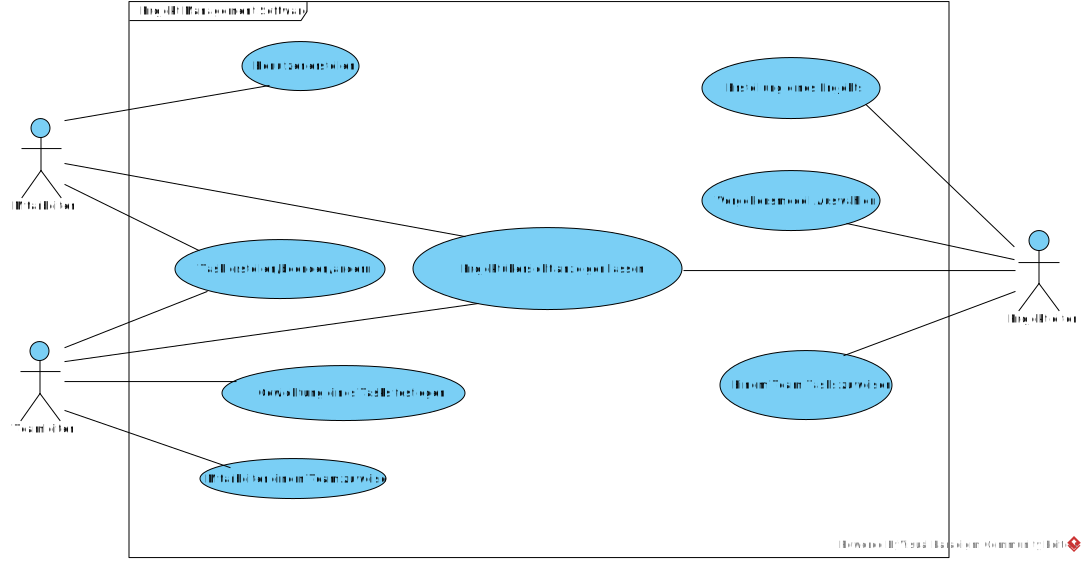
\includegraphics[width=\textwidth]{produktuebersicht.png}
% !TeX encoding=utf8
% !TeX spellcheck = de-DE

\section{Produktdaten}
\newcolumntype{s}{>{\hsize=.15\hsize}X}


\begin{tabularx}{\linewidth}{s X}
	\texttt{/D010/} & \textbf{Benutzerdaten}: Alle Daten die über einen Benutzer des Systems gespeichert werden.
	\begin{itemize}
		\item BenutzerID (eindeutig)
		\item Rolle (Entwickler, Projektleiter oder Teamleiter)
		\item Kennung \begin{itemize}
			\item Benutzername (eindeutig)
			\item Kennwort (verschlüsselt)
		\end{itemize}
		\item Name
		\item E-Mail Adresse
		\item Zugehörigkeit zu Teams (können mehrere sein)
	\end{itemize}
	\\
	 \texttt{/D020/} & \textbf{Teamdaten}: Alle Daten die die einzelnen Teams und ihre Zusammensetzung betreffen.
	 \begin{itemize}
	 	\item TeamID (eindeutig)
	 	\item Eine Liste der Teams
	 	\item Mitglieder der Teams und welchen Teams sie angehören.
	 	\item Teamleiter
	 	\item Den Teams zugeordnete Tasks
	 \end{itemize}
 	\\
 	 \texttt{/D030/} & \textbf{Projektdaten}: Alle Daten bezüglich laufender Projekte.
 	 \begin{itemize}
 	 	\item ProjektID (eindeutig)
 	 	\item Projektname
 	 	\item Dem Projekt zugewiesene Teams
 	 	\item Eine Beschreibung des Projekts
 	 	\item Das Ausgewählte Vorgehensmodell des Projekts. (Keins, Wasserfall, V-Modell, Spiralmodell)
 	 	\item Die Projektphasen entsprechend dem Vorgehensmodell \begin{itemize}
 	 		\item Aktuelle, nächsten und vorhergehenden Phasen
 	 	\end{itemize}
 	 \end{itemize}
	\\
\end{tabularx}
\clearpage
\begin{tabularx}{\linewidth}{s X}
	\texttt{/D040/} & \textbf{Task - Daten}: Alle Daten über Tasks welche in Bearbeitung, beendet oder geplant sind.
	\begin{itemize}
		\item TaskID (eindeutig)
		\item Deadline für die Task
		\item Zeitstempel an dem die Task abgeschlossen wurde
		\item Name und Beschreibung des Tasks
		\item Zugeteilte Projektphase(n)
		\item Abhängigkeiten und Reihenfolgen zu anderen Tasks
		\item Task Label
		\item Kommentare der Entwickler
	\end{itemize}
\end{tabularx}
\subsection{Datenbankschema}
\begin{figure*}[h!]
	\centering
	\includegraphics[width=0.65\textwidth]{owlkeeper_database.png}
\end{figure*}


% !TeX encoding=utf8
% !TeX spellcheck = de-DE

\section{Produktfunktionen}

% !TeX encoding=utf8
% !TeX spellcheck = de-DE

\section{Benutzeroberfläche}

\end{document}